\documentclass{standalone}
\usepackage{tikz}
\usetikzlibrary{automata,positioning,arrows,shapes,decorations,calc,
arrows.meta,fit}
\usetikzlibrary{decorations.pathmorphing}
\usetikzlibrary{decorations.pathreplacing}
\usetikzlibrary{decorations.shapes}
\usetikzlibrary{decorations.text}
\usetikzlibrary{decorations.markings}
\usetikzlibrary{decorations.fractals}
\usetikzlibrary{decorations.footprints}

\tikzset{
roundnode/.style={rectangle, draw=black, very thick, text width=20mm, minimum height=1cm},
phasenode/.style={rectangle, draw=black, very thick, text width=3cm, minimum height=1cm},
phasenodeBis/.style={rectangle, draw=black, very thick, minimum width=8cm, minimum height=5cm},
>={Latex[width=2mm,length=2mm]},
base/.style = {rectangle, rounded corners, draw=black,
                         minimum width=4cm, minimum height=1cm,
                         text centered, font=\sffamily},
%every picture/.style={/utils/exec={\sffamily}}
every edge quotes/.append style={font=\scriptsize, align=center, auto}% style for edge labels
}

\begin{document}
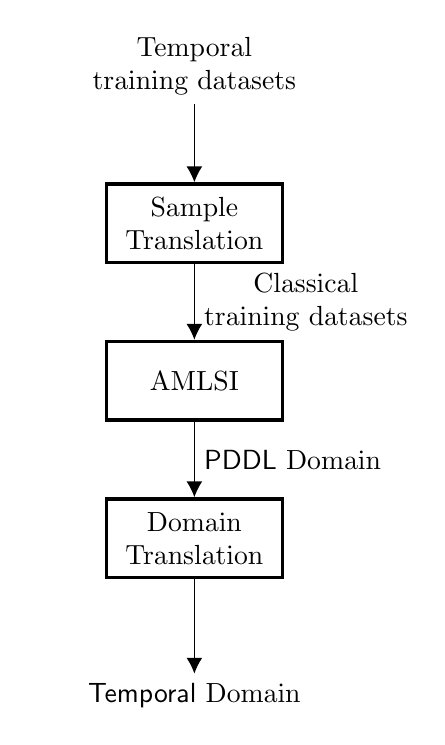
\begin{tikzpicture}[node distance=1.5cm, align=center]

%Automaton nodes
% \node[phasenode] (phase) at(2.5,3)  {\textbf{Phase I: Initialization phase}};
% \node[phasenodeBis] (phase2Bis) at(0,-1.5)  {};
\node[roundnode] (amlsi) at(0,4)  {AMLSI};
\node[roundnode] (sampleConv) at(0,6)  {Sample Translation};
\node[roundnode] (domainConv) at(0,2)  {Domain Translation};

\node[text width=4cm] (data) at(0,8)  {Temporal\\training datasets};
\node[text width=4cm] (output) at(0,0)  {{\sf Temporal} Domain};

\draw[->] (data) -- (sampleConv) ;
\draw[->] (sampleConv) --node[right] {Classical\\training datasets} (amlsi) ;
\draw[->] (amlsi) --node[right] {{\sf PDDL} Domain} (domainConv) ;
\draw[->] (domainConv) -- (output) ;
% \draw[->] (post) -- (output) ;
% \node (iteration) at(0,-1.25)  {$t^{th}$ iteration};

% \draw[->] (batch) --node[left] {} (grammar.north west) ;
% \draw[->] (initial.south) --node[right] {} (phase.north) ;
% \draw[->] (phase.south) --node[right] {Initial Domain $D^0$} (grammar.north east) ;
% \path[->] (grammar.east) edge[bend left] node[right] {Updated\\ Grammar} (overhaul.north) ;
% \draw[->] (overhaul.west) --node[below] {Overhauled\\ Domain $D^t$} (refinement.east) ;
% \path[->] (refinement.north) edge[bend left] node[left] {Refined\\ Domain $D^t$} (grammar.west) ;

% \draw [decorate,decoration={brace,amplitude=10pt,mirror,raise=6pt},yshift=0pt] (-4,-3.15) -- (4,-3.15);

% \node (phase2) at(0, -3.7) {\textbf{Phase II: Incremental learning process}};
% \node (output) at(0, -5) {Accurate PDDL Domain $D^t$ after convergence};
%
% \draw[->] (phase2Bis.south) -- (output.north) ;
\end{tikzpicture}
\end{document}
